\begin{frame}
    \frametitle{Body biasing injection: LIRMM BBI platform}
%    Generateur
    \begin{textblock*}{40mm}(5mm, 20mm)
        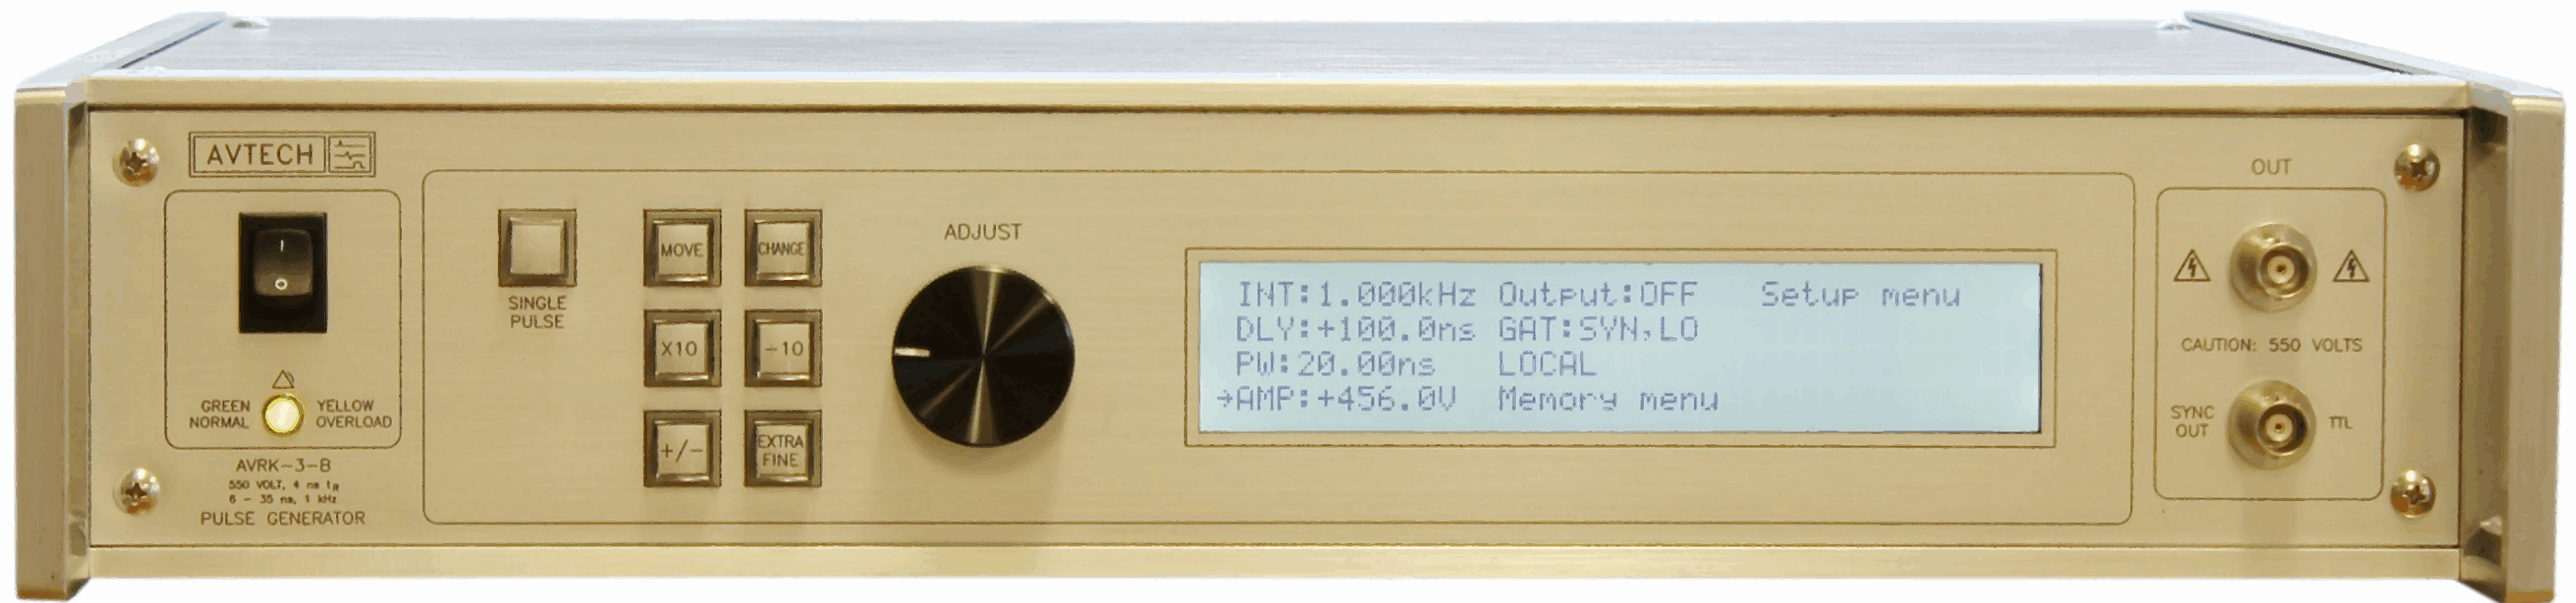
\includegraphics[width=\textwidth]{avrk4b.pdf}
    \end{textblock*}
%    Fleche generateur bas
    \begin{textblock*}{1mm}(24mm, 30mm)
        \begin{tikzpicture}
            \draw[-Stealth, blue, line width=0.5mm] (0, 0) -- (0, -1);
        \end{tikzpicture}
    \end{textblock*}
%    SOnde Loin
    \begin{textblock*}{30mm}(10mm, 42mm)
        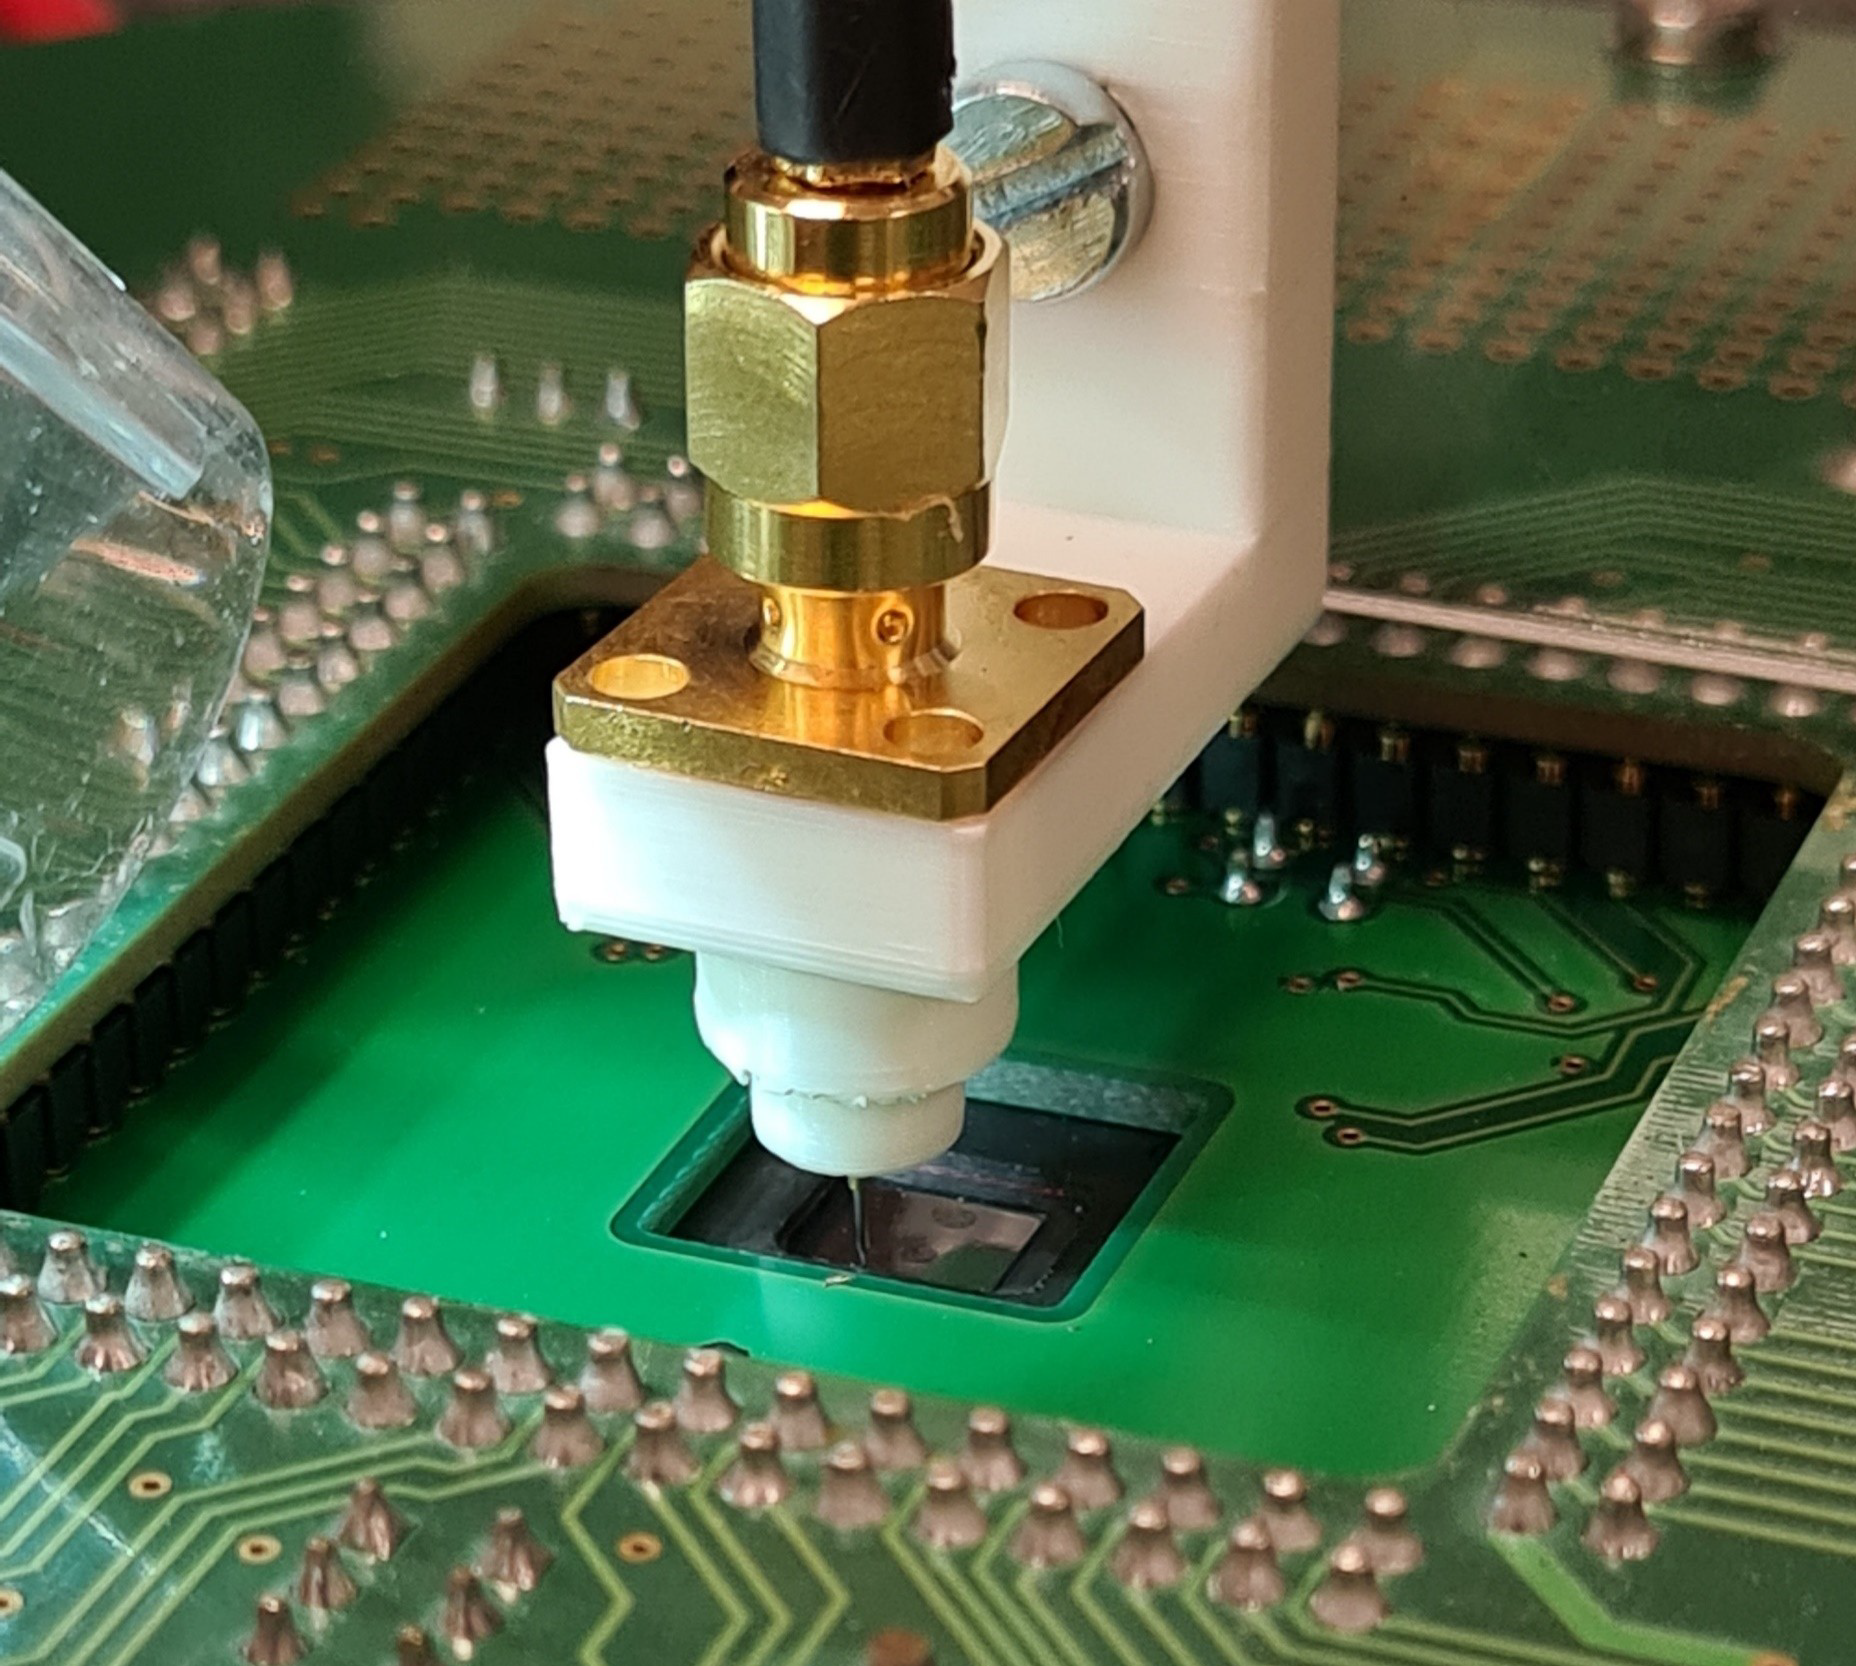
\includegraphics[width=\textwidth]{sondeBBI_loin_raw.png}
    \end{textblock*}
%    Fleche sonde loin droite
    \begin{textblock*}{1mm}(25.7mm, 63mm)
        \begin{tikzpicture}
            \draw[-Stealth, blue, line width=0.5mm] (0, 0) -- (1.8, -1);
        \end{tikzpicture}
    \end{textblock*}
%    Cercle sonde loin
    \begin{textblock*}{1mm}(21mm, 59mm)
        
\begin{tikzpicture}
            \draw[line width=0.5mm, color=blue] circle (0.25);
        \end{tikzpicture}
    \end{textblock*}
%    SOnde proche
    \begin{textblock*}{30mm}(47mm, 59mm)
        \includegraphics[width=\textwidth]{pointeBBI2.png}
    \end{textblock*}
%%    Fleche sonde proche droite/haut
%    \begin{textblock*}{1mm}(90mm, 48.5mm)
%        \begin{tikzpicture}
%            \draw[-Stealth, blue, line width=0.5mm] (0, 0) -| (1, 1.5);
%        \end{tikzpicture}
%    \end{textblock*}

%    Header Tableau
    \begin{textblock*}{1mm}(85mm, 18mm)
        \textbf{\underline{Main platform characteristics:}}
    \end{textblock*}
%    Tableau
    \begin{textblock*}{1mm}(85mm, 21mm)
%        Main platform characteristics
        \begin{table}[]
            \begin{tabular}{|
                    >{\columncolor[HTML]{34CDF9}}c |
                    >{\columncolor[HTML]{FFFFFF}}c |}
                \hline
                {\color[HTML]{000000} $V_{PULSE}$} & {\color[HTML]{000000} [150 ; 750] V} \\ \hline
                $P_W$                              & [6 ; 20] ns                          \\ \hline
                $T_R|T_F$                          & 4 ns                                 \\ \hline
                Recovery time                      & 1 ms                                 \\ \hline
                Propagation delay                  & 150 ns                               \\ \hline
                Input jitter                       & $\pm \; 100 \; ps \pm 0.03 \%$       \\ \hline
                Output coupling                    & DC                                   \\ \hline
                $Gen. \; I_{MAX}$ (50 \textOmega)  & 16 A                                 \\ \hline
                $Probe \; I_{MAX}$                 & 3 A                                  \\ \hline
                Probe \diameter                    & 40 µm                                \\ \hline
            \end{tabular}
        \end{table}
    \end{textblock*}
\end{frame}

\section*{THESIS OBJECTIVES}
\begin{frame}
    \frametitle{Thesis objectives}
    \begin{itemize}
        \setlength\itemsep{1em}
        \item What is the spatial resolution of BBI?
        \item What is the time resolution of BBI?
        \item Is thinning the substrate useful in any way?
        \item How BBI induced faults occur?
        \item How to model BBI?
    \end{itemize}
\end{frame}

\section*{THESIS AGENDA}
\begin{frame}
    \frametitle{Thesis agenda}
    \begin{itemize}
        \setlength\itemsep{1em}
        \item Enhancing the practice of Body Biasing Injection
        \item Integrated circuits modeling for BBI
        \item Enhanced simulation flow
        \item Substrate thinning analysis in a BBI context
        \item Conclusion and perspectives
    \end{itemize}
\end{frame}
